\subsection{Architecture Overview}
The protocol's architecture is divided into three abstract entities: the owner, the manufacturer, and the device. Figure \ref{sztp-architecture} illustrates the protocol's architecture.
\begin{figure}[H]
	\centering
	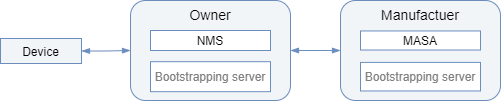
\includegraphics[scale=0.4]{Images/sztp-overview.png}
	\caption{SZTP Architecture.}
	\label{sztp-architecture}
\end{figure}
The owner is used to refer to the person or organization that owns the device. Throughout the protocol, the owner term abstractly represents the owner network domain and its sub-entities without explicitly referring to them. An example of the owner's sub-entities are the domain CA and the domain registrar. An owner possesses an \textit{Owner Certificate} which is an X.509 certificate that identifies the owner's identity and binds it to its public key. In addition to validating the owner's identity, the certificate is used to by other entities to validate the owner's digital signature over received artifacts. A \gls{nms} is assumed to be part of every owner's structure. A \gls{nms} is a software used by network administrators to monitor software and hardware nodes in a network and logs data from those nodes for reporting. The bootstrapping process introduces newly admitted devices to the \gls{nms}. 
\par
The manufacturer is the entity that produced the device. The term is also used to refer to entities that the manufacturer delegates functions to. A \gls{masa} is an example of a third party manufacturer delegate entity. Each manufacturer is supposed to operate a \gls{masa} or most commonly delegate its functionality to a third party. The \gls{masa} is responsible for generating the voucher required by the device to authenticate the owner and bootstrap the device. Each of the manufacturer services and its related entities has its own certificate for authentication and signing. The manufacturer preserves a list of trusted voucher-signing authorities and well-known bootstrap servers. The shipped devices from the manufacturer are pre-configured with the list of trust anchors along with their own \gls{idevid} credentials. Owners are assumed to trust the same pre-configured trust anchors as the ones maintained by the manufacturer.
\par
The protocol defines three artifacts that are exchanged through out the protocol: Conveyed information, ownership voucher, and owner certificate. Those artifacts provide the device with all the required information needed for bootstrapping. The conveyed information is divided between redirect information and onboarding information.
Bootstrap servers are \gls{rstcnf} servers that provide bootstrapping artifacts to devices. Depending on the type of information a server provides, they could split into two types of servers: Redirect servers and Onboarding servers. Redirect servers only returns redirect information to clients while onboarding servers only return onboarding information. However, servers are not limited to mentioned categories only. There may exist a server that can provide both types on conveyed information.
\par
Redirect information redirects a device to another bootstrapping server. 
Redirect information encodes a list of bootstrap servers hostnames and an optional trust anchor certificate that the device can use to authenticate each bootstrap server with. Depending on the source, redirect information may be trusted or untrusted. It is trusted whenever obtained via a secure connection to a trusted bootstrap server or whenever it is signed by the device’s owners. Trusted redirect information is useful for enabling a device to establish a secure connection to a specified bootstrap server. Untrusted redirect information is useful for directing a device to a bootstrap server where signed data has been staged for it to obtain. Redirection acts as a guide for device to discover the bootstrapping servers capable of providing onboarding information.
\par
Onboarding information is a bundle of data required for a device to perform the bootstrapping process into the owner’s network. It includes information about the boot image a device is required to be running, an initial configuration a device must apply, and scripts to address arbitrary needs which the device must successfully execute. Onboarding information must be obtained from a trusted source, either through a secure connection to a trusted bootstrap source or the information obtained is signed by the device’s owner.
\par
Devices can obtain the needed bootstrapping data from various sources according to the owner's deployed infrastructure. However, The concern is focused on sources that can supply devices with the information in an automated manner. Here are examples of touchless bootstrapping sources.
\begin{itemize}

\item
A DNS server can be utilized as a form of a bootstrapping server. It is an attractive method for environments which already employ a DNS infrastructure. It does necessarily require communication with an internet-accessible third party DNS service. Using DNS as bootstrapping server is considered a touchless bootstrapping as it does not involve any external interaction. However, a DNS server is not a trusted source of bootstrapping information, even if DNSSEC \cite{dnssec} is used to authenticate the DNS records. The reason being that the device cannot verify if the returned domain belongs to its rightful owner. Therefore, the returned DNS records must either be signed for later verification by the device or the records must be processed provisionally.
\par
Devices supporting DNS server as a bootstrap server are offered two prioritized types of queries to the server: device-specific and device independent queries. Queries must first be attempted using multicast DNS before unicast DNS. A DNS response for the device-specific query can encode the three artifacts into the TXT records but the response must be signed. However, by DNS conventions, the size of signed data is large. Therefore, it is implausible for the signed onboarding information to fit the UDP-based DNS packet size. Thus, if signed onboarding is to be sent over DNS, it is expected to be transported over \gls{tcp} so as to handle the DNS TXT record size. Otherwise, only redirect information shall be returned. On the other hand, DNS response for device-independent queries does not support returning onboarding information because the DNS server is incapable of returning signed data in response to the device-independent query. Accordingly, only redirect information shall be returned.
\item
Similar to DNS servers, a DHCP server is another untrusted bootstrapping data source. It can be leveraged by deployments that already employ a DHCP infrastructure. However, a DHCP server is a limited bootstrapping source due to its lack of ability to transmit enough data to hold signed bootstrapping data. Nevertheless, a DHCP server can return to a device unsigned redirect information.
\item
Lastly, a specific bootstrap server can be deployed to provide bootstrapping data and receive data from devices. It is defined as a \gls{rstcnf} server that implements the YANG module described in \cite[Section~7]{sztp}. Moreover, it may be using \gls{tls} which may eliminate the requirement to sign the transmitted bootstrapping data if the bootstrap server is trusted. Otherwise, if the bootstrap server is not trusted by the device, the conveyed information must be signed or processed provisionally. Whether a bootstrap server is trusted or not depends on the device’s knowledge of the server’s trust anchor. A bootstrap server exposes two endpoints to communicate with devices. Namely, the ``get-bootstrapping-data” for devices to request bootstrapping data and the ``report-progress” for devices to report their bootstrapping process status back to the bootstrap server, such as warnings, errors, and the result of the process. A bootstrap server may be hosted by the owner or is an internet accessible server hosted by the manufacturer.


\end{itemize}
